\section{Chapter 2: When the next spill is only a matter of time. Learning in the pipeline industry.}

\begin{singlespace}
	\begin{quote}
		"...I'm not convinced [that there is a problem]. We haven't had any phone calls. I mean it's perfect weather out here--if it's a rupture someone's going to notice that, you know and smell it" -- quote from a regional manager during the costliest onshore pipeline spill in history \citet[p. 100]{NTSB2012}.
	\end{quote}
\end{singlespace}

From 1980 to 2000, the US pipeline industry was a on a good track toward making pipelines safe. The standardized spill volume of refined petroleum pipelines more than halved, from a value of about 40 bbl per billion barrel-miles transported in 1980 to a value of below 20 in the last three years of the 20th century. Since the turn of the millennium, the standardized spill volume has been remarkable stable at a value of around 10 bbl per billion barrel-miles--so stable one can barely see a trend when fitting a curve (see Figure 2). After the year 2000, the development of new pipeline safety technology did not stop--but the trend of improving pipeline safety did come to an end. The end of a learning process is well known in the literature on \textit{organizational learning}. The theory of \textit{learning curves} is built on the assumption that the efforts of an organization to optimize a performance measure will end up looking like a distinct curve that initially falls quickly before learning declines \citep{Argote2013-1}. Figure 2 shows that pipeline safety follows the same pattern. 

{\noindent}\dotfill

\centerline{Insert Figure 2 about here}

{\noindent}\dotfill

\begin{figure}
	\caption{Pipeline safety improvements at the industry level for refined petroleum pipelines}
	\centerline{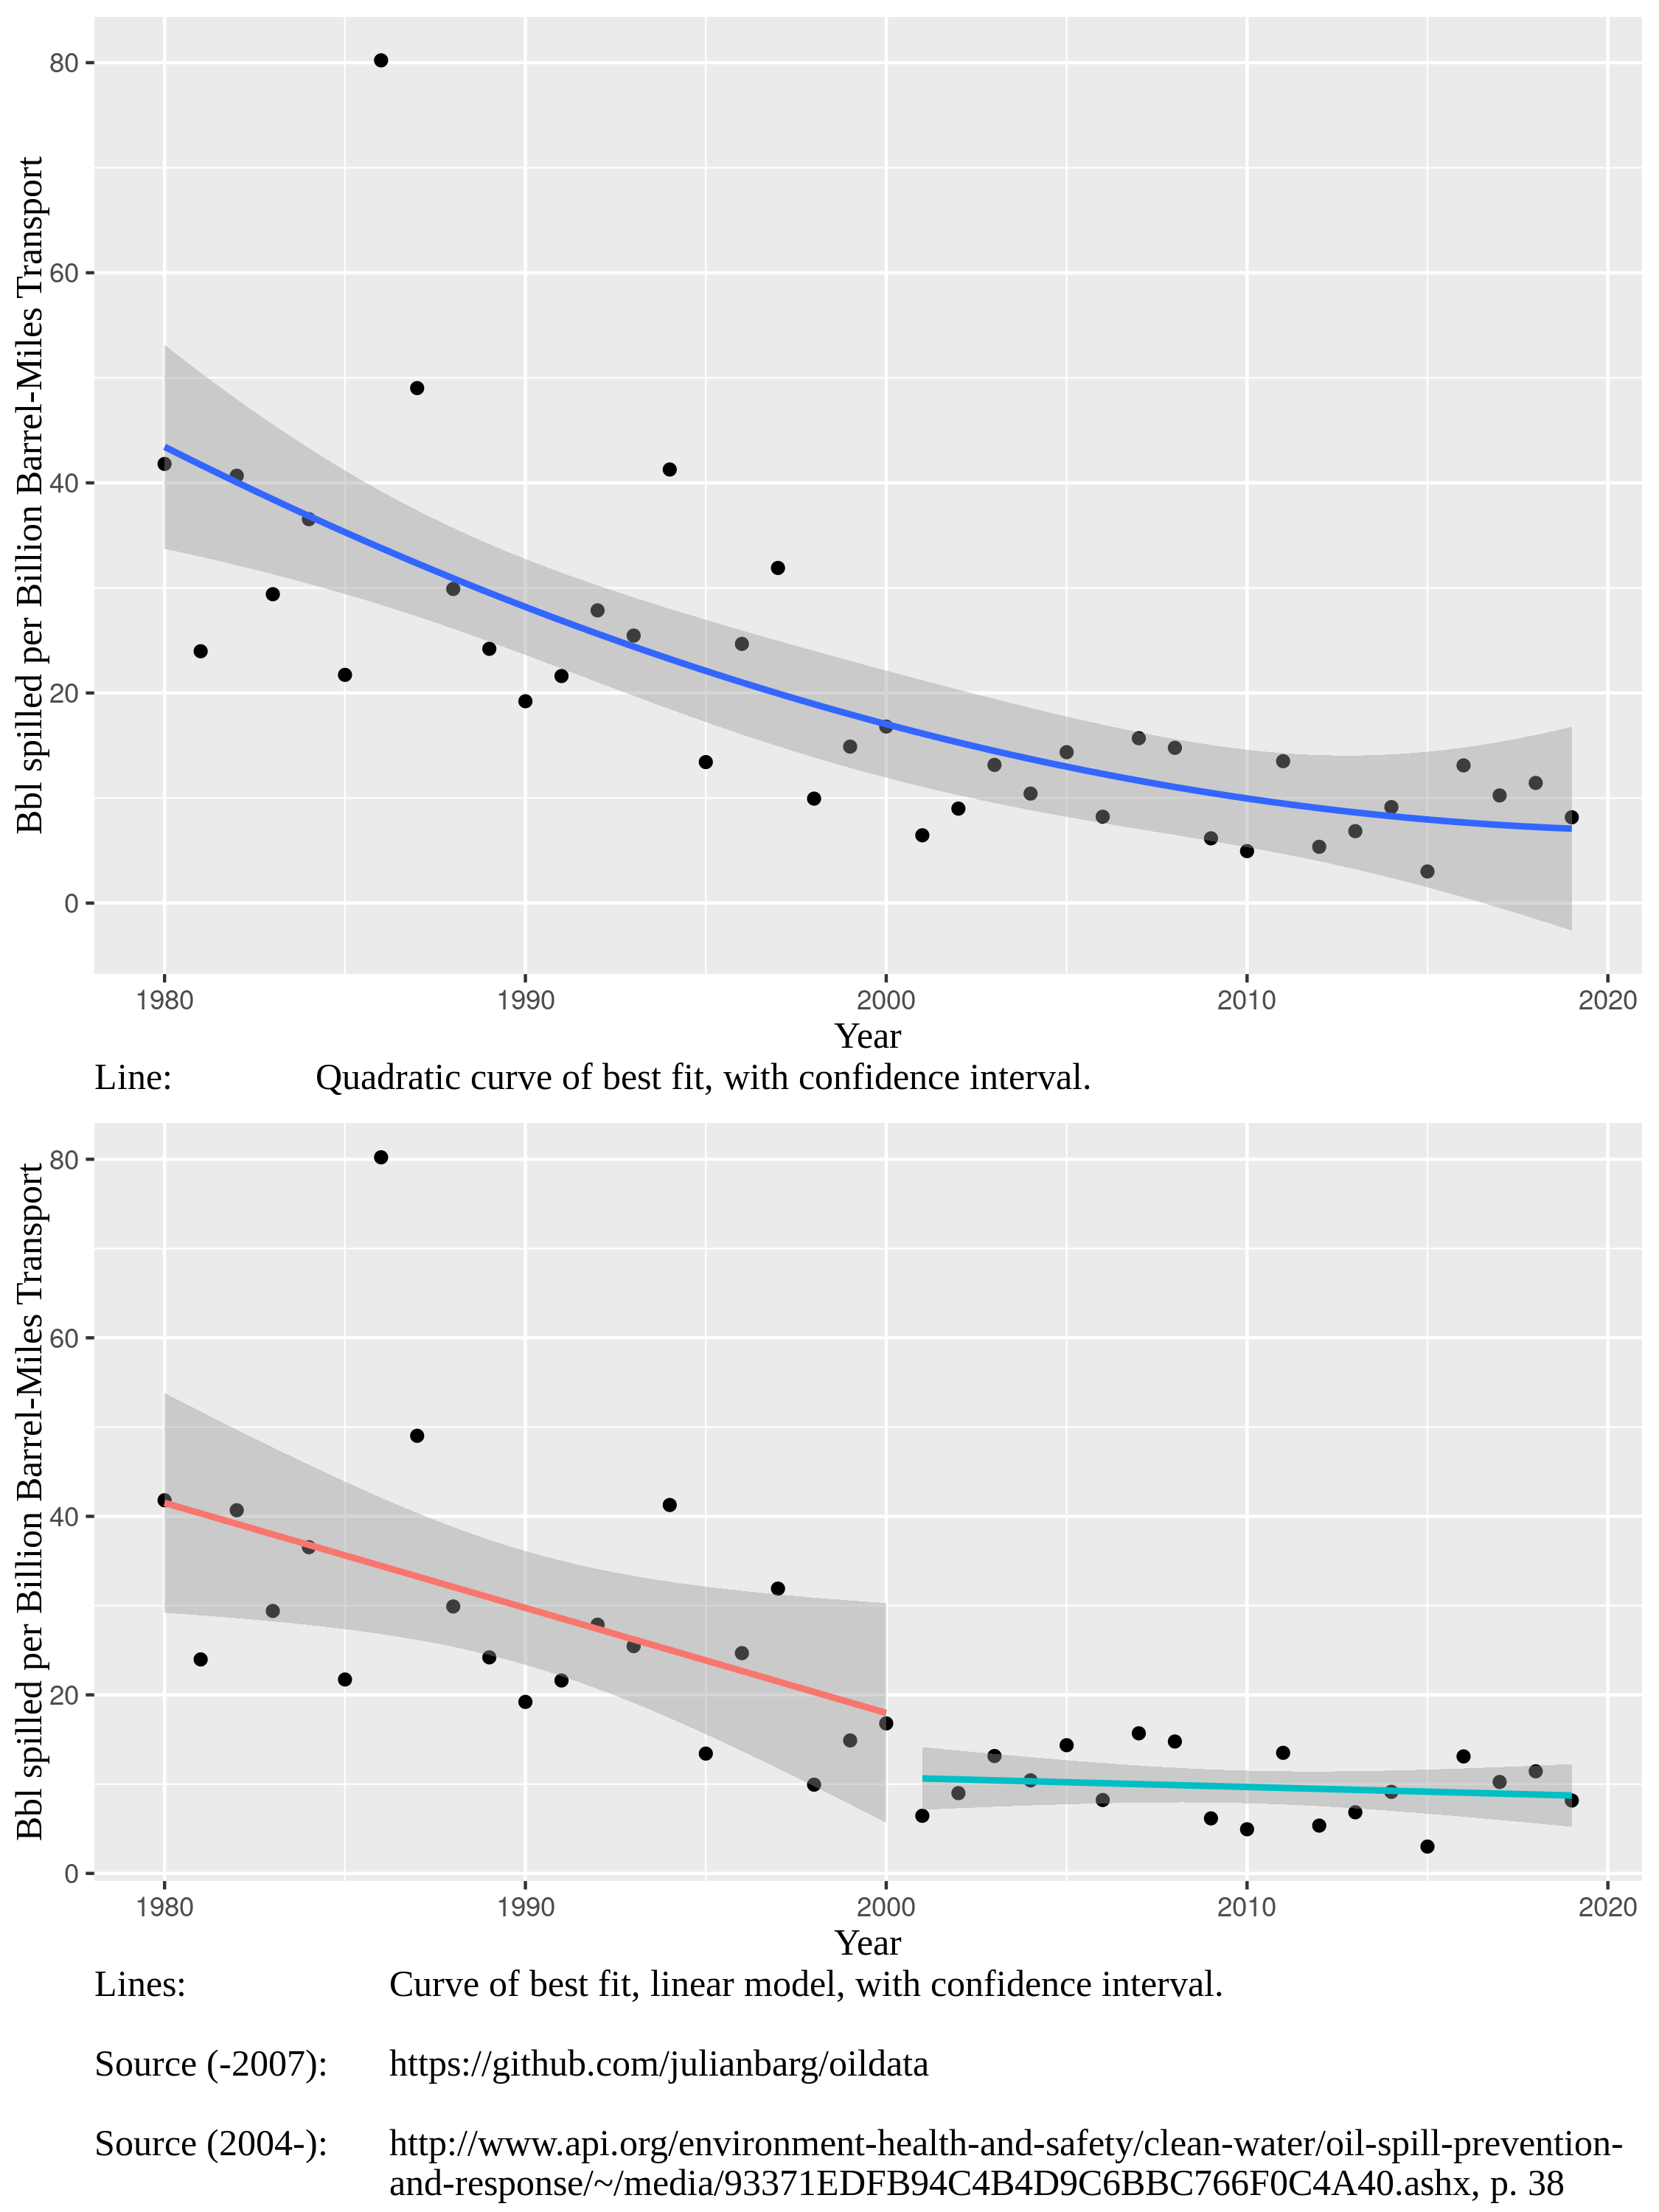
\includegraphics{../illustrations/population_learning_6.png}}
\end{figure}

The literature on organizational learning largely focuses on three issues: improvements of performance measures other than labor hours per unit of production (which the early literature focused on), knowledge transfer or vicarious learning, and organizational forgetting \citep{Argote2013-1}. This research does speaks to the first point, learning toward a diverse set of outcome variables, but it is not the focus of this work and the evidence is already quite compelling that organizations learn and improve any performance measures they track. Evidence is also conclusive that organizations learn vicariously from other similar others \citep{Kim2007}. The last point, organizational forgetting, has received less attention to date. Organizational forgetting paints a decisively less straightforward picture of organizational learning than the literature that precedes it. The concept acknowledges that learning is not always linear, and highlights that organizational dynamics have a bearing on knowledge \citep{Argote2013-3}.

If we take the learning curve seriously, we would expect that rapid improvements of performance measures are the exception, rather than the norm. Not on the organizational level, but on the level of a business unit or individual products or technologies, we would expect organizations to only spend a short time in a period of rapid improvements. Most of the time is spent in the tail end of the learning curve, where only marginal improvements are achieved, if any.\footnote{Conversation with colleagues always yields a lot of anecdotal evidence for this.} Organizational learning offers little in the way of explaining the process by which learning comes to a standstill.The literature currently has a a strong focus on \textit{organizational knowledge} \citep{Bingham2011}, from which we can derive two possible explanations. Either organizational knowledge eventually reaches a point of saturation, where the organization has attained an almost perfect command of the process. Or organizational forgetting could be a mechanism of convergence in learning. If an organization was to forget at the same pace as it is learning, that could give the impression of stagnation. This research will discuss the question head on: \textit{how does the convergence of a performance measure take place?}

This research takes a mixed-methods approach to uncover what happens inside organizations after the phase of rapid learning. The qualitative section takes a deductive approach. The qualitative data directly reveals that and how learning takes place in the pipeline industry, which is in the "long tail" of the learning curve. The quantitative section explains how the observation of learning in the pipeline industry is compatible with an absence of aggregate improvements of the performance measure. The qualitative section takes advantage of the well-established link between failure and learning \citep{Kim2007, Baum2007}. Failures are an unambiguous form of performance feedback and a strong catalysts for learning. Failure allows organizations to identify inadequate assumptions that underlie their activities, and develop models that better represent the world \citep{Madsen2010}. Pipeline spills act as looking glasses for this research, highlighting the problems that still exist in the management of pipeline safety and magnifying the actions taken by the industry and individual actors alike. The qualitative section is based on a sample of ten recent, significant pipeline spills. The quantitative section uses a dataset of the Pipeline and Hazardous Materials Safety Administration (PHMSA) on pipeline operators and spills. For the period from 2004-2019, this dataset holds information on 6,146 spills, including 2,246 that PHMSA deems significant. This research utilizes the textual descriptions of the spills in conjunction with spill rates to show that pipeline spills do trigger learning, but that pipelines have developed into complex systems that again and again surface unexpected interactions which lead to spills. To process that text data, I employ Topic Modeling \citep{Hannigan2019}. Difference-in-difference is used to show that learning still takes place in the pipeline industry in response to pipeline spills, despite a stagnation of pipeline safety.

Whilst the main contribution of this research is to shed light on the convergence stage of learning that arguably most organizations are in most of the time, the relevance of this research extends beyond just this phenomenon. The learning literature might give off impression that organizational learning is impactful and commonplace, when the reality might be that organizations run into limits all the time. Organizational learning might be the exception rather than the rule. By highlighting the limitations of conventional organizational learning, this research underlines the importance of learning that goes beyond optimizing performance measures. Something that the \textit{organizational knowledge} literature does not capture well is possibility to attain ones goal in a nonlinear fashion, for instance by questioning or abandoning currently held knowledge. With regard to attaining for example the viability or sustainability of a business unit, this research underlines the importance of exploration \citep{March1991}. For example, if society were to decide that the current pollution from pipelines spills is unacceptable, but that instead spill levels should be significantly lower, the trajectory that this research has identified suggests that pipeline operators or energy systems would need to make a radical departure from the current approach. The same could be the case for other systems with significant environmental impacts. Hence, this research also speaks to the discourse on \textit{grand challenges}: rather than highlighting individual contributions, this research alerts us to general trends. Here, literature on nonlinear learning can offern valuable insights \citep[e.g.,][]{Argyris1978, March2010}, as will be laid out in the discussion section.

%By understanding what happens in organizations . But potentially also what we can do about it. Is the process inevitable?

%will contribute of an understanding what we can do about it

%Organizational learning comes down to choices. Firms can either invest in improving existing technology, or develop new technology \citep{March1991}. Investing in the "wrong" technology can lead to technological lock-ins \citep{Levinthal1993}. The actors in the pipeline industry have selected a number of technological solutions to resolve their most pressing issue. When a pipeline spill occurs, the oil quickly infiltrates the soil and seeps into the groundwater.\footnote{The infiltration depth in sand is assumed to be over 10m in the first day alone \citep{Bonvicini2015}.} The environmental degradation caused by oil affects the local environment, and the local populace, too: a 2019 sibling comparison study on oil spills in Nigeria found that in localities that are affected by oil spills, for every 1,000 live births, an additional 38.3 neonatal deaths occur\citep{Bruederle2019}. % Potentially add impact of spills on industry? Stigmatized industry.

%In their fight against pipeline spills, pipeline operators employ a variety of technologies, such as smart pigs, leak detection systems, and SCADA systems. Smart pigs, while traveling through the pipes, utilize electromagnetic flux or ultrasonic probing to assess corrosion or mechanical damages to the pipe \citep{Singh2017-7}. Internal leak detection systems measure the flow of oil at two points A and B to detect any loss in between those points. External leak detection systems detect signs of escaping hydrocarbons, and include acoustic, hydrocarbon, and temperature sensors. \citep{Shaw2012}. SCADA systems are computer systems that allow an operator remotely monitor and operate lines. The operator typically sees on his screen charts of the flow at different points, can open and close valves, and startup or shutdown delivery of oil. Alarms from leak detection systems of the line are also displayed to the SCADA operator.\footnote{Larger pipeline companies operate control centers where all lines in a region are managed. Operators usually operate multiple SCADA systems at once, and more experienced employees supervise the operators. Control centers are operated in formal hierarchy, where for certain operations (such as clearing an alarm), a SCADA operator will require the go-ahead from a supervisor. See \citet{NTSB2012} for an in-depth description of an Enbridge control center in Edmonton as of 2012.}

%The high technology character of leak detection stands in contrast to the experienced reality of pipeline spills. A 2012 study commissioned by the Pipeline and Hazardous Materials Safety Administration (PHMSA) of onshore pipeline spills that occurred over a 19 month period, SCADA systems assisted in less than 25\% of cases with the detection and confirmation of the spill \citep[p. 3-33]{Shaw2012}. In only 17\% of cases was the operator or SCADA system listed as the initial identifier of the leak, while the public or emergency responders identified 30\% of leaks \citep[p. 3-39]{Shaw2012}. Why do the great learning efforts by pipeline operators fail to deliver the safety improvements that one would expect to see? A 2012 report prepared by the National Transportation Safety Board (NTSB) on the Kalamazoo River oil spill provides a good starting point for understanding the problem. A regional manager of Enbridge is quotes as saying: "...I'm not convinced [that there is a problem]. We haven't had any phone calls. I mean it's perfect weather out here--if it's a rupture someone's going to notice that, you know and smell it" \citep[p. 100]{NTSB2012}.

%This chapter uses the quantitative data from PHMSA to demonstrate how existing problems are addressed, following major spills that catch the attention of the industry, the regulator, and the public. That empirical observation is contrasted with the character of the two challenges that remain: (1) as holes are plugged, new unique sources of spills, for example climate change-related weather changes, emerge. (2) Both the "human factor" and the "organizational factor" are pervasive factors that yet to be completely eliminate as sources of error in any context. Overall, the geographic, technological, and organizational complexity of pipelines have led to the current situation, a quasi-standstill in the sector for refined oil. Crude oil pipelines on the other hand still have some potential for improvements, as simple and fundamental problem of this sector-- the corrosiveness of the commodity-- is addressed through new coatings, and cathodic protection.

%The quantitative section of this chapter uses a sample consisting of the 100 largest operators in the pipeline industry over the period from 2004 through 2019. The data that is available from PHMSA is matched and supplemented with data from Compustat. This quantitative section focuses on improvements over time in organizations affected by a specific source of incidents, and a reduction in certain causes of spills. Some qualitative data supplements the quantitative analysis by showcasing the processes of population level learning \citep{Miner1999}, especially for crude pipelines. The qualitative section then uses archival data to explore a sample of 15 major pipeline spills since 1986 to contrast the specificity of learning in the quantitative analysis with the complexity of the systems that the incidents occur in, and the complex interactions that lead to spills. The sample of 15 spills includes the top three spills with regard to spill volume, net loss (spill volume minus volume recovered), number of injuries, number of fatalities, and property damage. This sampling method ensure both a variety in the type of spills, and a good availability of archival data.

%This chapter contributes to the literature on knowledge-based learning by exploring the topic of a bottomed-out learning curve through raising the issue of aggregate and specific learning. The chapter also contributes to the debate on industry resource use: it discusses both the historical development and the potential future reduction (or lack thereof) of an industry's environmental footprint. Whereas in the past, improvements were made through incremental learning in the form of development of new technology, the analysis suggest that further improvements may only be possible through bold, maybe costly new choices, including a change of industry for some companies.

%Our qualitative analysis reveals that pipeline spills have all the hallmarks of normal accidents in complex systems \citep{Perrow1984}. Almost no two serious spills are alike, and the causes are as complex as the diverse political and physical environments that is the United States. Here, organizational learning is at an impasse. When efforts is made, and learning takes place, why do we not observe corresponding results? \citet{Levitt1988} propose that there are limitations to learning by doing. In those cases, learning cannot be disaggregated into its components. Instead, we need to look at the technological choices and determine whether an organization or industry has ended up in a competency trap \citep{Levitt1988}. An important factor for diagnosing this issue are feedback mechanisms: at the population level, is the problem diagnosed, or not? If in an industry the lack of learning goes unnoticed or is not addressed on a population level, even if learning takes place on a case-by-case basis, aggregate learning may not take place {MarchOlsen}.   

%With this article, we provide an additional perspective to the learning literature. Our interpretation of the data puts into question the notion of aggregate improvements through incremental, smaller scale learning. Instead, there are more substantive, technological improvements to be made, that sometimes cannot be attained through regular learning mechanisms. In those cases, a big picture perspective on the problem or goal is necessary to made a difference.

%   Other contribution: write something on learning that fills the gap created by publication bias.

%	Hints at a problem in the learning literature. Focusing on incremental improvement.

%   Claim quantitatie data as part of initial qualitative research? We looked at 10 major spills and x years of spill data, to understand how population-level learning works. Also, claim data on population level learning as part of the research.

%	Qualitative research approach--select spills--move through spills until motives saturated.

%	Limited ability to triangulate--but that is fine because our qualitative results are quite robust, and not too complex--little chance they are wrong.

%	Another omission that we decided on for this article are flaws in the environmental feedback mechanism, akin to those predicted in \citet{March1975}. Pipeline operators are well-insulated from the consequences of their actions, as the regulator (PHMSA) is understaffed and generally gives pipeline operators the benefit of doubt [provide evidene from NTSB].

